\part{ФОРМИРОВАНИЕ ШУМА}
    \setcounter{section}{0}
    \section{Описание процесса формирования шума}
        Интервал распределения шума задан как $ (-\Delta y; \Delta y) $, где коэффициент $\Delta y$ вычисляется по формуле:
        $$
            \Delta y = max(|y^{T}|) \cdot
            \begin{Bmatrix}
                0,05 \\
                0,1 \\
                0,2
            \end{Bmatrix}
            =
            \begin{Bmatrix}
                1.092 \\
                2.184 \\
                4.367
            \end{Bmatrix}
        $$

        После вычисления значений шума, необходимо добавить их к теоретическим значениям в интересующих нас точках для получения экспериментальных значений.

        Можно составить блок-схему процесса генерации экспериментальных значений.

        \begin{center}
            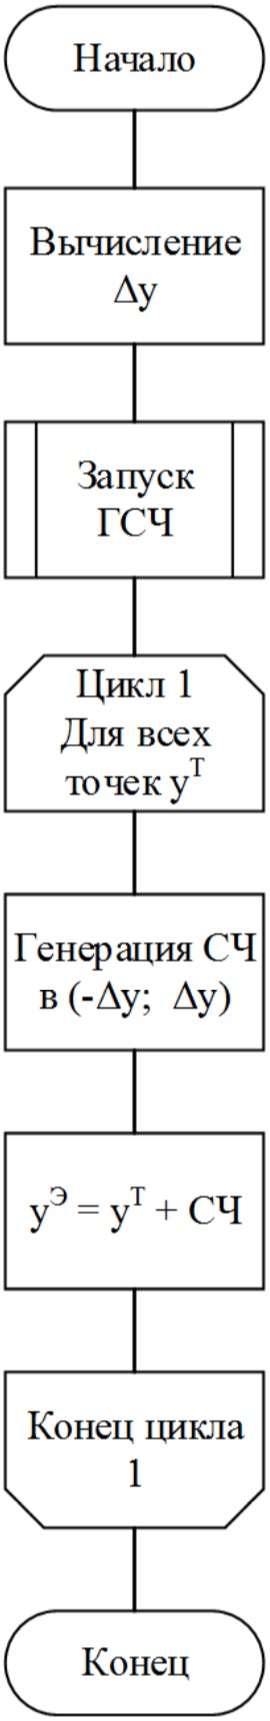
\includegraphics[scale=0.25]{img/block}
        \end{center}

    \section{Проверка ГСЧ}
        \begin{center}
            \begin{tikzpicture}
                \begin{axis}[ybar, ymin=0, ymax=1200]
                    \addplot [fill, color=blue] table [col sep=comma] {data/rnd.csv};
                    Гистограммы отражают исправную работу ГСЧ.
                \end{axis}
            \end{tikzpicture}
        \end{center}

    \section{Построим графики экспериментальных функций}
        \begin{tikzpicture}
            \begin{axis}
                \addplot table [col sep=comma] {data/theor.csv};
                \addplot table [col sep=comma] {data/noised005.csv};
            \end{axis}
        \end{tikzpicture}
        \begin{tikzpicture}
            \begin{axis}
                \addplot table [col sep=comma] {data/theor.csv};
                \addplot table [col sep=comma] {data/noised01.csv};
            \end{axis}
        \end{tikzpicture}

        \begin{center}
            \begin{tikzpicture}
                \begin{axis}
                    \addplot table [col sep=comma] {data/theor.csv};
                    \addplot table [col sep=comma] {data/noised02.csv};
                \end{axis}
            \end{tikzpicture}
        \end{center}
